% $Id: ArrayHalo_desc.tex,v 1.5 2006/02/07 20:25:05 nscollins Exp $

\label{sec:halo}
Halo operations update ghost cell or halo regions at the boundaries
of a local data decomposition.  Halo regions are to be considered
read-only by the local process; their data values can be used to
compute the new values for cells which are local to this process,
but they cannot be updated except by a halo operation.  Haloing is
supported at the Array and Field level.  The description of halo
regions that follows is phrased in terms of Arrays, but also holds
for Fields (which contain Arrays).

\subsection{Halo Domains}

Array objects can have an optional {\bf halo width} which defines
what part of the Array is the {\bf exclusive domain}, the {\bf computational
domain}, and the {\bf total domain}.  With no halo region, all these are
the same and equal to the total size of the Array.  The domains are
defined as follows.

\begin{itemize}

\item {\bf Exclusive}  The exclusive domain is the subset of the
Array which is never read by any other DE.  

\item {\bf Computational}  The computational domain
is the subset of the Array which is read and written by the current DE.

\item {\bf Total}  The total domain includes the region where data is 
updated from another DE during a halo operation and read but not 
updated by the current DE.  

\end{itemize}

Figure \ref{fig:halo} illustrates these concepts.

Halo domain information must be stored at the Array level to
support operations such as the gather, which collects
decomposed parts of a logically contiguous object onto a single DE.
Only the computational domain is copied since the halo regions are
duplicated data.  The exclusive domain is guaranteed to never be
the source of data for a halo operation, so no synchronization
of updates to those data items needs to be done.  The total
domain is the actual memory size allocated for the Array,
and is used when computing offsets for subdomains within the Array.

\begin{center}
\begin{figure}
\caption{Diagram showing how ESMF exclusive, computational,
and total domains are defined.  }
\label{fig:halo}
\scalebox{1.0}{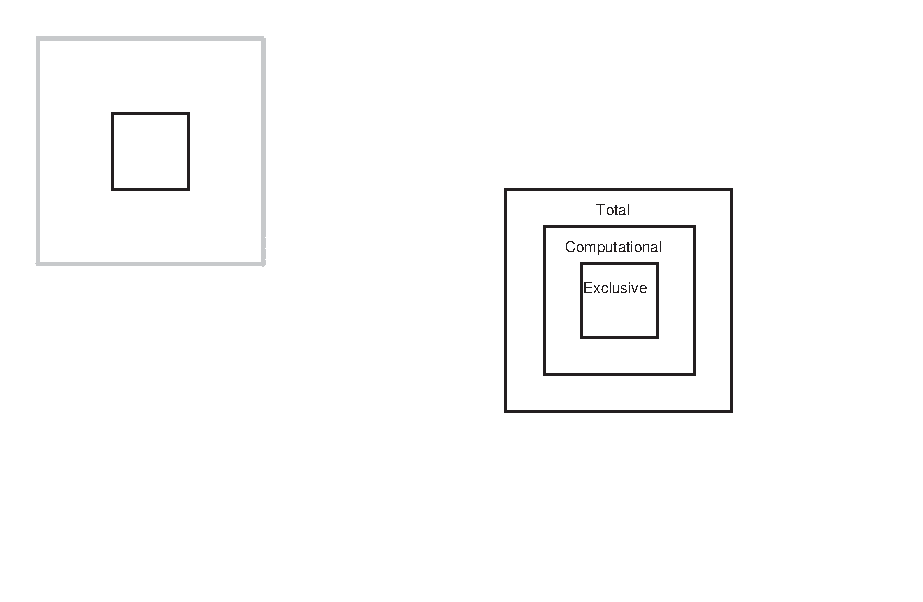
\includegraphics{Field_halo}}
\end{figure}
\end{center}


